\documentclass[11pt,a4paper,headinclude,footinclude,DIV16,normalheadings]{scrreprt}
\usepackage[automark]{scrpage2}
\usepackage[ansinew]{inputenc}
\usepackage{amsmath}
\usepackage{amsfonts}
\usepackage{theorem}
\usepackage{color}
\usepackage{listings}
\lstset{language=C++, basicstyle=\ttfamily, 
  keywordstyle=\color{black}\bfseries, tabsize=4, stringstyle=\ttfamily,
  commentstyle=\it, extendedchars=true, escapeinside={/*@}{@*/}}
\usepackage{hyperref}
\usepackage{psfrag}
\usepackage{makeidx}
\usepackage{graphicx}
\usepackage[htt]{hyphenat}
\usepackage{color}

\DeclareGraphicsExtensions{.eps, .jpg}

\newcommand{\Dune}{{\sf\bfseries DUNE}}
\newcommand{\Dumux}{DuMu$^\text{x}$ }

%The theorems
\theorembodyfont{\upshape}
\theoremheaderfont{\sffamily\bfseries}
\newtheorem{exc}{Exercise}[chapter]
\newtheorem{rem}[exc]{Remark}
\newtheorem{lst}{Listing}
\newtheorem{warn}[exc]{Warning}

\pagestyle{scrheadings}

\title{\Dumux Handbook}

\author{}

\date{\today}

\publishers{%
\vspace{10mm}
{\normalsize Lehrstuhl f\"ur Hydromechanik und Hydrosystemmodellierung, \\
Universit\"at Stuttgart, Paffenwaldring 61, D-70569 Stuttgart, Germany}\\
%
\bigskip
{\normalsize \texttt{\url{http://www.dumux.uni-stuttgart.de}}}\\
}

\makeindex

\begin{document}

\maketitle

\begin{abstract}

\end{abstract}

\tableofcontents

\chapter{Introduction}

\Dumux aims to be a generic framework for simulation of multiphase
fluid flow and transport processes in porous media using contiuum
mechanical approaches.  At the same time, \Dumux aims to deliver
top-notch computational performance, high flexibility, a sound
software architecture and the ability to run on anything from single
processor systems to highly parallel supercomputers with specialized
hardware architectures.

The means to achieve these somewhat contradictory goals are the
thorough use of object oriented design in conjunction with template
programming. These requirements lead to C++ as the implementation
language.

One of the more complex issues when dealing with parallel continuum
models is managing the grids used for the spatial discretization of
the physical model. To date, no generic and efficient approach exists
for all possible cases, so \Dumux is build on top of DUNE, the
\textbf{D}istributed and \textbf{U}nified \textbf{N}umerics
\textbf{E}nvironment~\cite{DUNE-HP}. DUNE provides a generic interface
to many existing grid management libraries such as UG~\cite{UG-HP},
ALBERTA~\cite{ALBERTA-HP}, ALU-Grid~\cite{ALUGRID-HP} and a few
more. DUNE also extensively uses template programming in order to
achieve minimal overhead when accessing the underlying grid
libraries\footnote{In fact, the performance penalty resulting from the
  use of DUNE's grid interface is usually
  negligible~\cite{BURRI2006}.}.
\begin{figure}[hbt]
  \centering 
  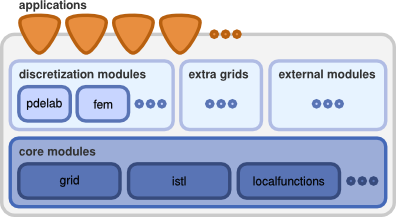
\includegraphics[width=.5\linewidth, keepaspectratio]{EPS/dunedesign}
  \caption{
    \label{fig:dune-design}
    A high-level overview on DUNE's design as available on the project's
    web site~\cite{DUNE-HP}.
  }
\end{figure}

DUNE's grid interface is independent of the spatial dimension of the
underlying grid. For this purpose, it uses the concept of
co-dimensional entities. Roughly speaking, an entity of co-dimension
$0$ constitutes a cell, co-dimension $1$ entities are faces between
cells, co-dimension $1$ are edges, and so on until co-dimension $n$
which are the cell's vertices.  The DUNE grid interface generally
assumes that all entities are convex polytopes, which means that it
must be possible to express each entity as the convex hull of a set of
vertices. For efficiency, all entities are further expressed in terms
of so-called reference elements which are transformed to the actual
spatial incarnation within the grid by a so-called geometry
function\footnote{The same approach is also used by \texttt{dune-disc} for
  finite element shape functions.}. Here, a reference element for an
entity can be thought of as a prototype for the actual grid
entity. For example, if we used a grid that used hexahedrons as cells,
the reference element for each cell would be the unit cube $[0, 1]^3$
and the geometry function would scale and translate the cube so that
it matches the grid's cell. For a more thorough description of DUNE's
grid definition, see~\cite{BASTIAN2008}.

In addition to the grid interface, DUNE also provides quite a few
additional modules, of which the \texttt{dune-pdelab},
\texttt{dune-localfunctions} and \texttt{dune-istl} modules are the
most relevant in the context of this handbook.  \texttt{dune-pdelab}
provides a toolbox for discretization and includes matrix assemblers
for translating local stiffness matrices into a global linear system
of equations and much more, while \texttt{dune-localfunctions}
provides a set of generic finite element shape
functions. \texttt{dune-istl} is the \textbf{I}terative
\textbf{S}olver \textbf{T}emplate \textbf{L}ibrary and provides
generic, highly optimized linear algebra routines for solving the
generated systems.

\Dumux comes in form of an additional module \texttt{dumux}. 
It depends on the DUNE core modules 
\texttt{dune-common}, \texttt{dune-grid}, \texttt{dune-istl}, \texttt{dune-localfunctions}, as well as from 
the discretization module \texttt{dune-pdelab}. 
The main intention of \Dumux is to provide a framework for easy and efficient 
implementation of new physical models for porous media flow problems, 
ranging from problem formulation, the selection of 
spatial and temporal discretization schemes, as well as nonlinear solvers,  
up to general concepts for model coupling.  
Moreover, \Dumux includes ready to use numerical models and a few example applications. 


\chapter{Getting started}

We first describe the steps which are necessary for installing DuMu$^\text{x}$ 
and then provide a quick start guide for the first DuMu$^\text{x}$ experience. 
We conclude this chapter with a copy of the DUNE coding guidelines. 

\section{Installation of \Dumux} \label{install}
\subsection{Preliminary remarks}

In this section about the installation of \Dumux it is assumed that you work on a UNIX or Linux compatible operating system
and that you are familiar with the use of a command line shell. Installation means that you unpack \Dune together with \Dumux in a certain directory.
Then, you compile it in that directory tree where you do the further work, too. You also should know how to install new software packages
or you should have a person aside which can give you assistance with that. In section \ref{sec:prerequisites} we list some prerequisites for running \Dune and \Dumux. 
Please check this paragraph whether you can fulfill them. In addition, section \ref{sec:external-modules-libraries} provides some details on optional libraries and modules.

In a technical sense \Dumux is a module of \Dune. 
Thus, the installation procedure of \Dumux is the same as that of \Dune. 
Details regarding the installation of \Dune are provided on the \Dune website \cite{DUNE-INST}. 
If you are interested in more details about the build system that is used,
they can be found in the {\Dune} Buildsystem Howto \cite{DUNE-BS}.


All \Dune modules including \Dumux get extracted into a common directory, as it is done in a usual \Dune installation. 
We refer to that directory abstractly as {\Dune} root directory or shortly as {\Dune}-Root. 
If it is used as directory's path of a shell command it is typed as \texttt{\Dune-Root}. 
For the real {\Dune} root directory on your file system any valid directory name can be chosen.

Source code files for each \Dune module are contained in their own subdirectory within {\Dune}-Root.
We name this directory of a certain module ``module root directory" or \texttt{module-root-directory} if it is a directory path,
e.g. for the module \texttt{dumux} these names are  ``dumux root directory" respective \texttt{dumux-root-directory}.
The real directory names for modules can be chosen arbitrarily, in this manual they are the same as the
module name or the module name extended by a version number suffix.
The name of each \Dune module is always defined in the file \texttt{dune.module}, which is in root
directory of the respective module. This should not be changed by the user. 
It is allowed to have own files and directories in \Dune-Root, which are not related to \Dune's needs.

After installing source code for all relevant \Dune modules including \Dumux, \Dune is being built by the shell-command \texttt{dunecontrol} which is part of the \Dune build system. The \Dune build system is a front-end of to the GNU build system adapted to the needs of \Dune.

\subsection{Prerequisites} \label{sec:prerequisites}
The GNU tool chain of \texttt{g++}  and the tools of the GNU build system \cite{GNU-BS}, also known as GNU autotools
(\texttt{autoconf}, \texttt{automake}, \texttt{autogen}, \texttt{libtool}), as well as the GNU variant of \texttt{make}
must be available in a recent version. For Ubuntu Linux, e.g.,  these are contained in the
packages \texttt{autoconf}, \texttt{automake}, \texttt{libtool}
and the C++ compiler \texttt{g++} and \texttt{make} are contained in \texttt{build-essential}.

At the time of writing this manual, it is expected that \texttt{g++} of version $\geqslant$ 4.4.1, \texttt{automake} of version $\geqslant$ 1.11,
\texttt{autoconf} of version $\geqslant$ 2.65, \texttt{autogen} of version $\geqslant$ 5.9.7,  \texttt{libtool} of version $\geqslant$ 2.2.6
and GNU \texttt{make} version $\geqslant$ 3.81 should do their job for building \Dumux.
\Dumux makes use of the \texttt{boost} library in the version $\geqslant$ 1.33.1, but optional external modules may require a more recent version. 
It is thus necessary to install an appropriate developer package of \texttt{boost}
which is sometimes also named \texttt{libboost}. The matching Ubuntu Linux package is \texttt{libboost-dev}.

The building of included documentation like this handbook requires \LaTeX\  and auxiliary tools
like \texttt{dvipdf} and \texttt{bibtex}. One usually chooses a \LaTeX\  distribution like \texttt{texlive} for doing that.
It is possible to switch off the building of the documentation by setting the switch \texttt{--disable-documentation} 
in the \texttt{CONFIGURE\_FLAGS} of the building options (see Chapter \ref{buildIt}).
Additional parts of documentation are contained within the source code files as special formatted comments.
Extracting them can be done with \texttt{doxygen} (version $\geqslant$ 1.7.2 works). 
See for this optional step Section \ref{sec:build-doxy-doc}.

Depending on whether you are going to use external libraries and modules for additional \Dune features, 
additional software packages may be required. Some hints on that are given in Section \ref{sec:external-modules-libraries}.

For the extraction of the content of tar-files, the GNU version of \texttt{tar} is used.
The subversion (svn) software repositories can be accessed with help of a subversion client. We recommend the Apache Subversion command-line client \texttt{svn}
contained in Apache Subversion of version $\geqslant$ 1.6.0 \cite{APACHE-SUBVERSION-HP}. 

\subsection{Obtaining source code for \Dune and \Dumux}
As stated before, the \Dumux release 2.0 is based on the \Dune release 2.0, comprising the core modules 
\texttt{dune-common}, \texttt{dune-grid}, \texttt{dune-istl}, \texttt{dune-localfunctions} and the external dune
module \texttt{dune-pdelab}. Thus, for a proper \Dumux installation these modules are required.

Two possibilities exist to get the source code of \Dune and \Dumux.
Firstly, \Dune and \Dumux can be downloaded as tar-files from the respective {\Dune} and {\Dumux} website. They have to be extracted as described in the next paragraph.
Secondly, a method to obtain the most recent source code (or more generally any of its the previous revisions) by direct access 
via Internet to the software repositories of the revision control system is described in the subsequent part. 

However, if a user does not want to use the most recent version,
certain version tags (i.e. special names), version numbers and even software branches are means 
of the software revision control system to provide access to different versions of the software.

\paragraph{Obtaining the software by installing tar-files}
The slightly old-fashioned named tape-archive-file shortly named tar-file or tarball is a common file format for distributing collections of files contained within these archives.
The extraction from the tar-files is done as follows: 
Download the tarballs from the respective \Dune (version 2.0) and \Dumux websites to a certain folder in your file system.
Create the {\Dune} root directory, named DUMUX in the example below. Then extract the content of the tar-files, e.g. with the command-line program \texttt{tar}.
This can be achieved by the following shell commands. Replace \texttt{path\_to\_tarball} with the directory name where the downloaded files are actually located.
After extraction, the actual name of the dumux root directory is \texttt{dumux-2.0}. 

\begin{lstlisting}[style=Bash]
$ mkdir DUMUX
$ cd DUMUX
$ tar xzvf path_to_tarball_of/dune-common-2.0.tar.gz 
$ tar xzvf path_to_tarball_of/dune-grid-2.0.tar.gz 
$ tar xzvf path_to_tarball_of/dune-istl-2.0.tar.gz 
$ tar xzvf path_to_tarball_of/dune-localfunctions-2.0.tar.gz 
$ tar xzvf path_to_tarball_of/dumux-2.0.tar.gz
\end{lstlisting}

Furthermore, if you wish to install the optional \Dune Grid-Howto which provides a tutorial on the Dune grid interface:

\begin{lstlisting}[style=Bash]
$ tar xzvf path_to_tarball_of/dune-grid-howto-2.0.tar.gz
\end{lstlisting}

However, the required \Dune-module \texttt{dune-pdelab} is not available as tar-file.
It can be installed from a software repository via svn.
If \texttt{svn} is available in the command line, it can be done as follows: 

\begin{lstlisting}[style=Bash]
$ svn co https://svn.dune-project.org/svn/dune-pdelab/branches/2.0snapshot dune-pdelab
\end{lstlisting}

\paragraph{Obtaining \Dune and \Dumux from software repositories} 

Direct access to a software revision control system for downloading code can be of later advantage for the user. 
It can be easier for him to keep up with code changes and to receive important bug fixes using the update command of the revision control system. 
\Dune and \Dumux use Apache Subversion for their software repositories. To access them a certain program is needed which is referred here shortly as subversion client. 
In our description, we use the subversion client of the Apache Subversion software itself, which is a command-line tool named \texttt{svn}. 
It is available for most Linux and UNIX distributions as software package.

In the technical speech of Apache Subversion ``checking out a certain software version" means nothing more then fetching 
a local copy from the software repository and laying it out in the file system.  Additionally to the software some more files for the use of the software revision control system itself are created. They are kept in directories named \texttt{.svn} and can be found in each subfolder that is under version control.
If you have developer access to \Dumux, it is also possible to do the opposite, i.e. loading up a modified revision of software into the software repository. This is usually termed as ``software commit".

The installation procedure is done as follows:
Create a  {\Dune} root directory, named DUMUX in the lines below.
Then, enter the previously created directory and check out the desired modules. 
As you see below, the check-out uses two different servers for getting the sources, one for \Dune and one for {\Dumux}.
The \Dune modules of the stable 2.0 release are checked out as described on the \Dune website \cite{DUNE-DOWNLOAD-SVN}:

\begin{lstlisting}[style=Bash]
$ mkdir DUMUX
$ cd DUMUX
$ svn co https://svn.dune-project.org/svn/dune-common/releases/2.0 dune-common
$ svn co https://svn.dune-project.org/svn/dune-grid/releases/2.0 dune-grid
$ svn co https://svn.dune-project.org/svn/dune-istl/releases/2.0 dune-istl
$ svn co https://svn.dune-project.org/svn/dune-localfunctions/releases/2.0 dune-localfunctions
$ svn co https://svn.dune-project.org/svn/dune-pdelab/branches/2.0snapshot dune-pdelab
\end{lstlisting}

The newest (unstable) developments are also provided in these repositories, usually in a folder called ``trunk''. Please check the \Dune website \cite{DUNE-DOWNLOAD-SVN} for further information. However, the current \Dumux release is based on the stable 2.0 release and it will not compile without further adaptations using the the newest versions of \Dune.

The additional module \texttt{dune-grid-howto} is a tutorial which provides information about the \Dune grid interface.
It may give you an idea how some abstractions in \Dune are done.
The \texttt{dune-grid-howto} is not required by \Dumux, the installation is optional. It is done by: 

\begin{lstlisting}[style=Bash]
$ svn co https://svn.dune-project.org/svn/dune-grid-howto/releases/2.0 dune-grid-howto
\end{lstlisting}

The \texttt{dumux} module is checked out as described below (see also the \Dumux website \cite{DUMUX-HP}).
Its file tree has to be created in the \Dune-Root directory, where the \Dune modules are also have been checked out to. Subsequently, the next command
is executed there, too. The dumux root directory is called \texttt{dumux} here.

\begin{lstlisting}[style=Bash]
$ # make sure you are in DUNE-Root
$ svn co --username=anonymous --password='' svn://svn.iws.uni-stuttgart.de/DUMUX/dumux/trunk dumux
\end{lstlisting}

\paragraph{Hints for \Dumux-Developers}
If you also want to actively participate in the development of \Dumux, you can apply either for full developer
access or for developer access on certain parts of \Dumux. Granted developer access means that
you are allowed to commit own code and that you can access the \texttt{dumux-devel} module.
This enhances \texttt{dumux} by providing (unstable) code from the developer group.
A developer usually checks out non-anonymously the modules \texttt{dumux} and \texttt{dumux-devel}. 
\texttt{Dumux-devel} itself makes use of the stable part \texttt{dumux}. Hence, the two parts have to be checked out together.
This is done by the commands below. But \texttt{joeuser} needs to be replaced by
the actual user name of the developer for accessing the software repository. 
One can omit the \texttt{--username} option in the commands above, if the user name for the repository access is
identical to the one for the system account.

\begin{lstlisting}[style=Bash]
$ svn co --username=joeuser svn://svn.iws.uni-stuttgart.de/DUMUX/dumux/trunk dumux
$ svn co --username=joeuser svn://svn.iws.uni-stuttgart.de/DUMUX/dune-mux/trunk dumux-devel
\end{lstlisting}

Please choose either not to store the password by subversion in an insecure way or
choose to store it by subversion in a secure way, e.g. together with \texttt{kwallet} or \texttt{gnomekeyring}.
Check the documentation of subversion, how this is being done.
A leaked out password can be used by evil persons to abuse a software repository.

\paragraph{checkout-dumux script}
The shell-script \texttt{checkout-dumux} facilitates setting up a {\Dune}/{\Dumux} directory tree.
It is contained in the download section of the \Dumux web page \cite{DUMUX-HP}.
For example the second line below will check out the required \Dune modules and \texttt{dumux}, \texttt{dumux-devel} and the \texttt{external} folder, which contains some useful external software and libraries.
Again,  \texttt{joeuser} needs to be replaced by the actual user name.

\begin{lstlisting}[style=Bash]
$ checkout-dumux -h      # show help,
$ checkout-dumux -gme -u joeuser -p password -d DUMUX 
\end{lstlisting}

\subsection{Patching \Dune or external libraries}
Patching of \Dune modules in order to work together with \Dumux
can be necessary for several reasons.
Software like a compiler or even a standard library
changes at times. But, for example, a certain release of a software-component that we depend on, may not reflect that change and thus it has to be modified.
In the dynamic developing process of software that depends on other modules it is not always feasible 
to adapt everything to the most recent version of each module. Consequently, patches exist or they are be brought into existence. They may fix problems with a certain module
of a certain release without introducing too much structural change. It can also happen 
that a release gets amendments (updates) and a formerly useful patch becomes obsolete.

\Dumux contains patches and documentation about their usage and application within the directory \texttt{dumux/patches}.
Please check the README file in that directory for recent information. 
In general, a patch can be applied as follows (the exact command or the used parameters may be slightly different).

\begin{lstlisting}[style=Bash]
$ # make sure you are in DUNE-Root
$ cd dune-istl
$ patch -p1 < ../dumux/patches/dune-istl-2.0.patch
\end{lstlisting}

It can be removed by 
\begin{lstlisting}[style=Bash]
$ path -p1 -R < ../dumux/patches/dune-istl-2.0.patch
\end{lstlisting}

The \texttt{checkout-dumux} script also applies patches, if not explicitly requested to do not so.

\subsection{Build of \Dune and \Dumux}
\label{buildIt}
Building of \Dune and \Dumux is done by the command-line script \texttt{dunecontrol} as described in \Dune Installation Notes \cite{DUNE-INST}
and in much more comprehensive form in the \Dune Buildsystem Howto \cite{DUNE-BS}.
If something fails during the execution of \texttt{dunecontrol} feel free to report it to the \Dune or \Dumux developer mailing list,
but also try to include error details.\\

It is possible to compile \Dumux with nearly no explicit options to the build system.
%, but experience showed that the code quality through all parts of \Dune is not yet high enough to give the compiler full 
%freedom for allowing certain kind optimizations. 
However, for the successful compilation of \Dune and \Dumux, it is currently necessary to pass the
%As options, switches for the optimization can be set in parts
%build system for code by default, it is safer to pass 
the option \texttt{-fno-strict-aliasing} to the C++-compiler
\cite{WIKIPED-ALIASING}, which is done here via a command-line argument to \texttt{dunecontrol}:


\begin{lstlisting}[style=Bash]
$ # make sure you are in the directory DUNE-Root
$ ./dune-common/bin/dunecontrol --configure-opts="CXXFLAGS=-fno-strict-aliasing"  all
\end{lstlisting}

Too many options can make life hard, that's why usually option-files are being used together with dunecontrol and its sub-tools.
Larger sets of options are kept in them. If you are going to compile with options suited for debugging of the code, the following
can be a starting point:

%Below in command-line make sure to insert the right name of dumux' root directory, which is in case of installation from tar-files \texttt{dumux-2.0} or in case of installation from subversion just \texttt{dumux}. For a developer it is also possible to take options file from \texttt{dumux-devel}.

\begin{lstlisting}[style=Bash]
$ # make sure you are in the directory DUNE-Root
$ cp dumux/debug.opts my-debug.opts      # create a personal version
$ gedit my-debug.opts                    # optional editing the options file 
$ ./dune-common/bin/dunecontrol --opts=my-debug.opts all 
\end{lstlisting}

More optimized code, which is typically not usable for standard debugging tasks, can produced by 

\begin{lstlisting}[style=Bash]
$ cp dumux/optim.opts my-optim.opts 
$ ./dune-common/bin/dunecontrol --opts=my-optim.opts all
\end{lstlisting}

Sometimes it is necessary to have additional options which
are specific to a package set of an operating system or
sometimes you have your own preferences.
Feel free to work with your own set of options, which may evolve over time.
The option files above are more to be understood as a starting point
for setting up an own customization than as something which is fixed.
The use of external libraries can make it necessary to add quite many options in an option-file.
It can be helpful to give your customized option file its own name, as done above.
One avoids to confused it with the option files that came out of the distribution
and that can be possibly updated by subversion later on.

\subsection{Building doxygen documentation} \label{sec:build-doxy-doc}

Doxygen documentation is done by especially formatted comments integrated in the source code, which can get extracted by the program 
\texttt{doxygen}. Beside extracting these comments, \texttt{doxygen} builds up a web-browsable code structure documentation
like class hierarchy of code displayed as graphs, see \cite{DOXYGEN-HP}.

Building the doxygen documentation of a module is done as follows, provided the program \texttt{doxygen} is installed:
Set in building options the \texttt{--enable-doxygen} switch.
This is either accomplished by adding it in \texttt{dunecontrol} options-file to  \texttt{CONFIGURE\_FLAGS}, or by adding
it to  \texttt{dunecontrol}'s command-line-argument \texttt{--configure-opts}. 
After running \texttt{dunecontrol} enter in module's root directory the subdirectory \texttt{doc/doxygen}.
You then run the command \texttt{doxygen} within that directory. Point your web browser to the file 
\texttt{module-root-directory/doc/doxygen/html/index.html} to read the generated documentation.
All  \Dune-modules that are used here except \texttt{dune-grid-howto}  including also \texttt{dumux} contain some doxygen documentation, which can be extracted as
described in the following lines. The external library UG has also a \texttt{doc/doxygen} directory for building its doxygen documentation.

\begin{lstlisting}[style=Bash]
$ # change before next command your directory to DUNE-Root
$ cd dumux/doc/doxygen
$ doxygen
$ firefox html/index.html
\end{lstlisting}

\subsection{Building documentation of other \Dune modules}

If the \texttt{--enable-documentation} switch has been set in the configure flags of
\texttt{dunecontrol}, this does not necessarily mean that for every 
\Dune module the documentation is being build.
However, at least Makefiles for building the documentation are generated.
Provided you run \texttt{dunecontrol} with the option above,
it should be possible to build documentation if available.
Check in \texttt{module-root-directory/doc/Makefile.am} which targets you can build.
E.g., for the module \texttt{dune-istl} you can build the documentation \texttt{istl.pdf} by typing the following into the console, when you are in the \Dune-Root:

\begin{lstlisting}[style=Bash]
$ # change before next command your directory to DUNE-Root
$ cd dune-istl/doc
$ make istl.pdf
\end{lstlisting}

Or for module \texttt{dune-grid-howto} the documentation can be build by: 

\begin{lstlisting}[style=Bash]
$ # change before next command your directory to DUNE-Root
$ cd dune-grid-howto/doc
$ make grid-howto.pdf
\end{lstlisting}

This applies for \Dumux too. Rebuilding the handbook can be done as follows:

\begin{lstlisting}[style=Bash]
$ cd dumux/doc/handbook
$ make dumux-handbook.pdf
\end{lstlisting}


%At the time writing this to the author no general method of building documentation contained in \Dune's modules is known.

%Alternatively, the tool CMake can be used to build \Dumux. Please check the file \texttt{INSTALL.cmake} for details.

\subsection{External libraries and modules} \label{sec:external-modules-libraries}

The libraries described in the sequel of this paragraph provide additional functionality but are not generally required to run \Dumux. 
If you are going to use an external library check the information provided on the \Dune website \cite{DUNE-EXT-LIB}.
If you are going to use an external \Dune module the website on external modules \cite{DUNE-EXT-MOD} can be helpful.\\
%Further information on external modules and libraries seemed to be contained in {\Dune}s Wiki \cite{DUNE-MAIN-WIKI}.


Installing an external library can require additional libraries which are also used by \Dune. 
For some libraries, such as BLAS or MPI, multiple versions can be installed on system.
Make sure that it uses the same library as \Dune when configuring the external library.

In the following list, you can find some external modules and external libraries, and some more libraries and tools which are prerequisites for their use.

\begin{itemize}
\item \textbf{ALBERTA}: External library for use as GRID. Adaptive multi Level finite element toolbox using Bisectioning refinement and Error control by Residual Techniques for scientific Applications. Building it requires a FORTRAN compiler \texttt{gfortran}. Download: \texttt{\url{http://www.alberta-fem.de}}.

\item \textbf{ALUGrid}: External library for use as GRID. ALUGrid is build by a C++-compiler like \texttt{g++}. If you want to build a parallel version, you will need \texttt{MPI}. It was successfully run with \texttt{openmpi}. The parallel version needs also a graph partitioner, such as \texttt{METIS}. It was run successfully in combination with \Dune using \texttt{METIS}. \\
Download: \texttt{\url{http://aam.mathematik.uni-freiburg.de/IAM/Research/alugrid}}

\item \textbf{\Dune-multidomaingrid}: External module. If you going to run on the same grid different domains or subdomains,
this can be the package of choice. This is done by providing a meta grid. It can be useful for multi-physics approaches or domain decomposition methods. Download: \texttt{\url{http://gitorious.org/dune-multidomaingrid}}. 
%Furthermore, the external module \textbf{\Dune-multidomain} can be useful for solving heterogenous problems on spatial subdomains. These subdomains are managed using another DUNE module called dune-multidomaingrid.

\item \textbf{PARDISO}: External library for solving linear equations. The package PARDISO is a thread-safe, high-performance, robust, memory efficient and easy to use software for solving large sparse symmetric and asymmetric linear systems of equations on shared memory multiprocessors. The precompiled binary can be downloaded after personal registration from the PARDISO website (\texttt{\url{http://www.pardiso-project.org}}).

\item \textbf{SuperLU}: External library for solving linear equations. SuperLU is a general purpose library for the direct solution of large, sparse, non-symmetric systems of linear equations. \\ (\texttt{\url{http://crd.lbl.gov/~xiaoye/SuperLU}}).

\item \textbf{UG}: External library for use as GRID. UG is a toolbox for Unstructured Grids: For \Dumux it has to be build by GNU buildsystem and a C++-compiler. That's why \Dune specific patches need applied before use. Building it makes use of the tools \texttt{lex}/\texttt{yacc} or the GNU variants \texttt{flex}/\texttt{bison}. 

\end{itemize}

The following are dependencies of some of the used libraries. You will need them depending on which modules of \Dune and which external libraries you use.

\begin{itemize}
\item \textbf{MPI}: The parallel version of \Dune and also some of the external dependencies need MPI when they are going to be built for parallel computing. \texttt{Openmpi} version $\geqslant$ 1.4.2 and \texttt{MPICH} in a recent version have been reported to work. 

\item \textbf{lex/yacc} or \textbf{flex/bison}: These are quite common developing tools, code generators for lexical analyzers and parsers. This is a prerequisite for UG.

\item \textbf{BLAS}: Alberta makes use of BLAS. Thus install GotoBLAS2, ATLAS, non-optimized BLAS or BLAS provided by a chip manufacturer. Take care that the installation scripts select the intended version of BLAS. See \texttt{\url{http://en.wikipedia.org/wiki/Basic_Linear_Algebra_Subprograms}}.

\item \textbf{GotoBLAS2}: This is an optimized version of BLAS. It covers not always available all processors of the day, but quite a broad range. Its license is now very open.  A FORTRAN compiler like \texttt{gfortran} is needed to compile it.\\
Available by \texttt{\url{http://www.tacc.utexas.edu/tacc-projects/gotoblas2/}}.

\item \textbf{METIS}: This is a dependency of ALUGrid, if you are going to run it parallel.

\item \textbf{Compilers}: Beside \texttt{g++} it has been reported that \Dune was successfully build with the Intel C++ compiler. 
C and FORTRAN compiler is needed for a some external libraries. As code of different compilers is linked together they have to be be compatible with each other. A good choice is the GNU compiler suite \texttt{gcc},\texttt{g++} and \texttt{gfortran}.

\item \textbf{libgomp}: External libraries, such as ALUGrid, can make use of OpenMP when used together with METIS. For that purpose it can be necessary to install the \texttt{libgomp} library.
% http://openmp.org/

%\item \textbf{libgmp}: The Gnu Multiple Precision Arithmetic Library (GMP) is also a prerequisite for \Dune. It may be necessary to install it.
% http://gmplib.org/
\end{itemize}

\subsection{Hints for Users from IWS}
We provide some features to make life a little bit easier for
users from the Institute of Hydraulic Engineering, University of Stuttgart.

There exists internally a svn repository made for several external libraries.
If you are allowed to access it, go to the {\Dune}-Root, then do: 
\paragraph{prepared external directory}

\begin{lstlisting}[style=Bash]
$ # Make sure you are in DUNE-Root
$ svn checkout svn://svn.iws.uni-stuttgart.de/DUMUX/external/trunk external
\end{lstlisting}

This directory \texttt{external} contains a script to install external libraries, such as 
ALBERTA, ALUGrid, UG, METIS and GotoBLAS2: 

\begin{lstlisting}[style=Bash]
$ cd external
$ ./installExternal.sh all
\end{lstlisting}

It is also possible to install only the actual needed external libraries:

\begin{lstlisting}[style=Bash]
$ ./installExternal.sh -h      # show, what options this script provide
$ ./installExternal.sh --parallel alu
\end{lstlisting}

The libraries are then compiled within that directory and are not installed in a different place. 
A \Dune build may need to know their location. Thus, one may have to refer to them as options for \texttt{dunecontrol}, 
for example via the options file \texttt{my-debug.opts}.


\section[Quick start guide]{Quick start guide: The first run of a test application}\label{quick-start-guide}

The previous chapter showed, how to install and compile \Dumux. This chapter shall give a very brief introduction, how to run a first test application and how to visualize the first output files. Only the rough steps will be described here. More detailed explanations can be found in the tutorials in the following chapter.

\begin{enumerate}
 \item Go to the directory \texttt{dune-mux/test}. There, various test application folders can be found. Let us consider as example \texttt{test{\_}2p}:
 \item Enter the folder \texttt{2p}. If everyting was compiled correctly, there should be an executable \texttt{test{\_}2p}. In order to run the simulation, type\\ 
\texttt{./test{\_}2p 1e4 1e2}\\
into the console. The parameters that are used here are the end time of the simulation and the initial timestep size. The parameters that are required when calling the application are specified in the application file (here: test{\_}2p.cc).
 \item The simulation starts and produces some .vtu output files and also a .pvd file. The .pvd file can be used to examine time series and summarizes the .vtu-files. It is possible to stop a running application by pressing $<ctrl><c>$.
 \item You can display the results using the previously installed visualization tool ParaView (or alternatively VisIt). Just type \texttt{paraview} in the console and open the .pvd file. On the left hand side, you can choose the desired parameter to be displayed.
\end{enumerate}
% 
%
%



\section{Guidelines} 

This section mainly quotes the DUNE coding guidelines found at \cite{DUNE-HP}.
"In order to keep the code maintainable we have decided upon a set of coding rules. 
Some of them may seem like splitting hairs to you, but they do make it much easier 
for everybody to work on code that hasn't been written by oneself.

\begin{itemize}
\item Naming: 
\begin{itemize}
\item Variables: Names for variables should only consist of letters and digits. The first letter should be a lower case one. If your variable names consists of several words, then the first letter of each new word should be capital. As we decided on the only exception are the begin and end methods.
\item Private Data Variables: Names of private data variables end with an underscore.
\item Typenames: For typenames, the same rules as for variables apply. The only difference is that the first letter should be a capital one.
\item Macros: The use of preprocessor macros is strongly discouraged. If you have to use them for whatever reason, please use capital letters only.
\item The Exlusive-Access Macro: Every header file traditionally begins with the definition of a preprocessor constant that is used to make sure that each header file is only included once. If your header file is called 'myheaderfile.hh', this constant should be DUNE\_MYHEADERFILE\_HH.
\item Files: Filenames should consist of lower case letters exclusively. Header files get the suffix .hh, implementation files the suffix .cc
\end{itemize}
\item Documentation:
      Dune, as any software project of similar complexity, will stand and fall with the quality of its documentation.
Therefore it is of paramount importance that you document well everything you do! We use the doxygen system to extract easily-readable documentation form the source code. Please use its syntax everywhere. In particular, please comment all
\begin{itemize}
\item Method Parameters
\item Template Parameters
\item Return Values
\item Exceptions thrown by a method
 \end{itemize}
     Since we all know that writing documentation is not well-liked and is frequently defered to some vague 
'next week', we herewith proclaim the Doc-Me Dogma . It goes like this: Whatever you do, and in whatever hurry you 
happen to be, please document everything at least with a {\verb /** $\backslash$todo Please doc me! */}. That way at least the absence 
of documentation is documented, and it is easier to get rid of it systematically.
\item Exceptions:
      The use of exceptions for error handling is encouraged. Until further notice, all exceptions thrown are DuneEx.
\item Debugging Code:
      Global debugging code is switched off by setting the symbol NDEBUG. In particular, all asserts are 
automatically removed. Use those asserts freely!" 
\end{itemize}


\section[Quick start guide]{Quick start guide: The first run of a test application}\label{quick-start-guide}

The previous chapter showed, how to install and compile \Dumux. This chapter shall give a very brief introduction, how to run a first test application and how to visualize the first output files. Only the rough steps will be described here. More detailed explanations can be found in the tutorials in the following chapter.

\begin{enumerate}
 \item Go to the directory \texttt{dune-mux/test}. There, various test application folders can be found. Let us consider as example \texttt{test{\_}2p}:
 \item Enter the folder \texttt{2p}. If everyting was compiled correctly, there should be an executable \texttt{test{\_}2p}. In order to run the simulation, type\\ 
\texttt{./test{\_}2p 1e4 1e2}\\
into the console. The parameters that are used here are the end time of the simulation and the initial timestep size. The parameters that are required when calling the application are specified in the application file (here: test{\_}2p.cc).
 \item The simulation starts and produces some .vtu output files and also a .pvd file. The .pvd file can be used to examine time series and summarizes the .vtu-files. It is possible to stop a running application by pressing $<ctrl><c>$.
 \item You can display the results using the previously installed visualization tool ParaView (or alternatively VisIt). Just type \texttt{paraview} in the console and open the .pvd file. On the left hand side, you can choose the desired parameter to be displayed.
\end{enumerate}
% 
%
%



\chapter[Tutorial]{Tutorial}

In \Dumux two sorts of models are implemented: Fully coupled models, and decoupled models. In the fully coupled models a flow system is described by a system of strongly coupled equations which can be mass balance equations, balance equations of components, energy balance equations, etc. In contrast a decoupled model consists of a pressure equation which is decoupled or only weakly coupled to a saturation equation, concentration equations, energy balance equations, etc.

Different kinds of both coupled and decoupled models can be isothermal two phase models, isothemal two phase two component models, non-isothermal twophase model, non-isothermal two phase two component models, etc.

The following two sections of the tutorial demonstrate how to solve problems first using a coupled model (section \ref{tutorial-coupled}) and second using a decoupled model (section \ref{tutorial-decoupled}). Being the easiest case, a isothermal two phase system (two fluid phases, one solid phase) will be considered.
\clearpage
\section[Fully-coupled model]{Solving a problem using a Fully-Coupled Model}\label{tutorial-coupled}

The process of solving a problem using \Dumux can be roughly divided into four parts:
\begin{enumerate}
 \item The geometry of the problem and correspondingly a grid have to be defined.
 \item Material properties and constitutive relationships have to be defined.
 \item Boundary conditions as well as initial conditions have to be defined.
 \item A suitable model has to be chosen.
\end{enumerate}

The problem that is solved in this tutorial is illustrated in figure \ref{tutorial-coupled:problemfigure}. A rectangular domain with no flow boundaries on the top and on the bottom, which is initially saturated with oil, is considered. Water infiltrates from the left side into the domain. Gravity effects as well as capillarity effects are neglected.

\begin{figure}[h]
\psfrag{x}{x}
\psfrag{y}{y}
\psfrag{no flow}{no flow}
\psfrag{water}{\textbf{water}}
\psfrag{oil}{\textcolor{white}{\textbf{oil}}}
\psfrag{p_w = 2 x 10^5 [Pa]}{$p_w = 2 \times 10^5$ [Pa]}
\psfrag{p_w_initial = 2 x 10^5 [Pa]}{\textcolor{white}{\textbf{$\mathbf{p_{w_{initial}} = 2 \times 10^5}$ [Pa]}}}
\psfrag{S_n = 0}{$S_n = 0$}
\psfrag{S_n_initial = 0}{\textcolor{white}{$\mathbf{S_{n_{initial}} = 1}$}}
\psfrag{q_w = 0 [kg/m^2s]}{$q_w = 0$ $\left[\frac{\textnormal{kg}}{\textnormal{m}^2 \textnormal{s}}\right]$}
\psfrag{q_n = -3 x 10^-4 [kg/m^2s]}{$q_n = -3 \times 10^-4$ $\left[\frac{\textnormal{kg}}{\textnormal{m}^2 \textnormal{s}}\right]$}
\centering
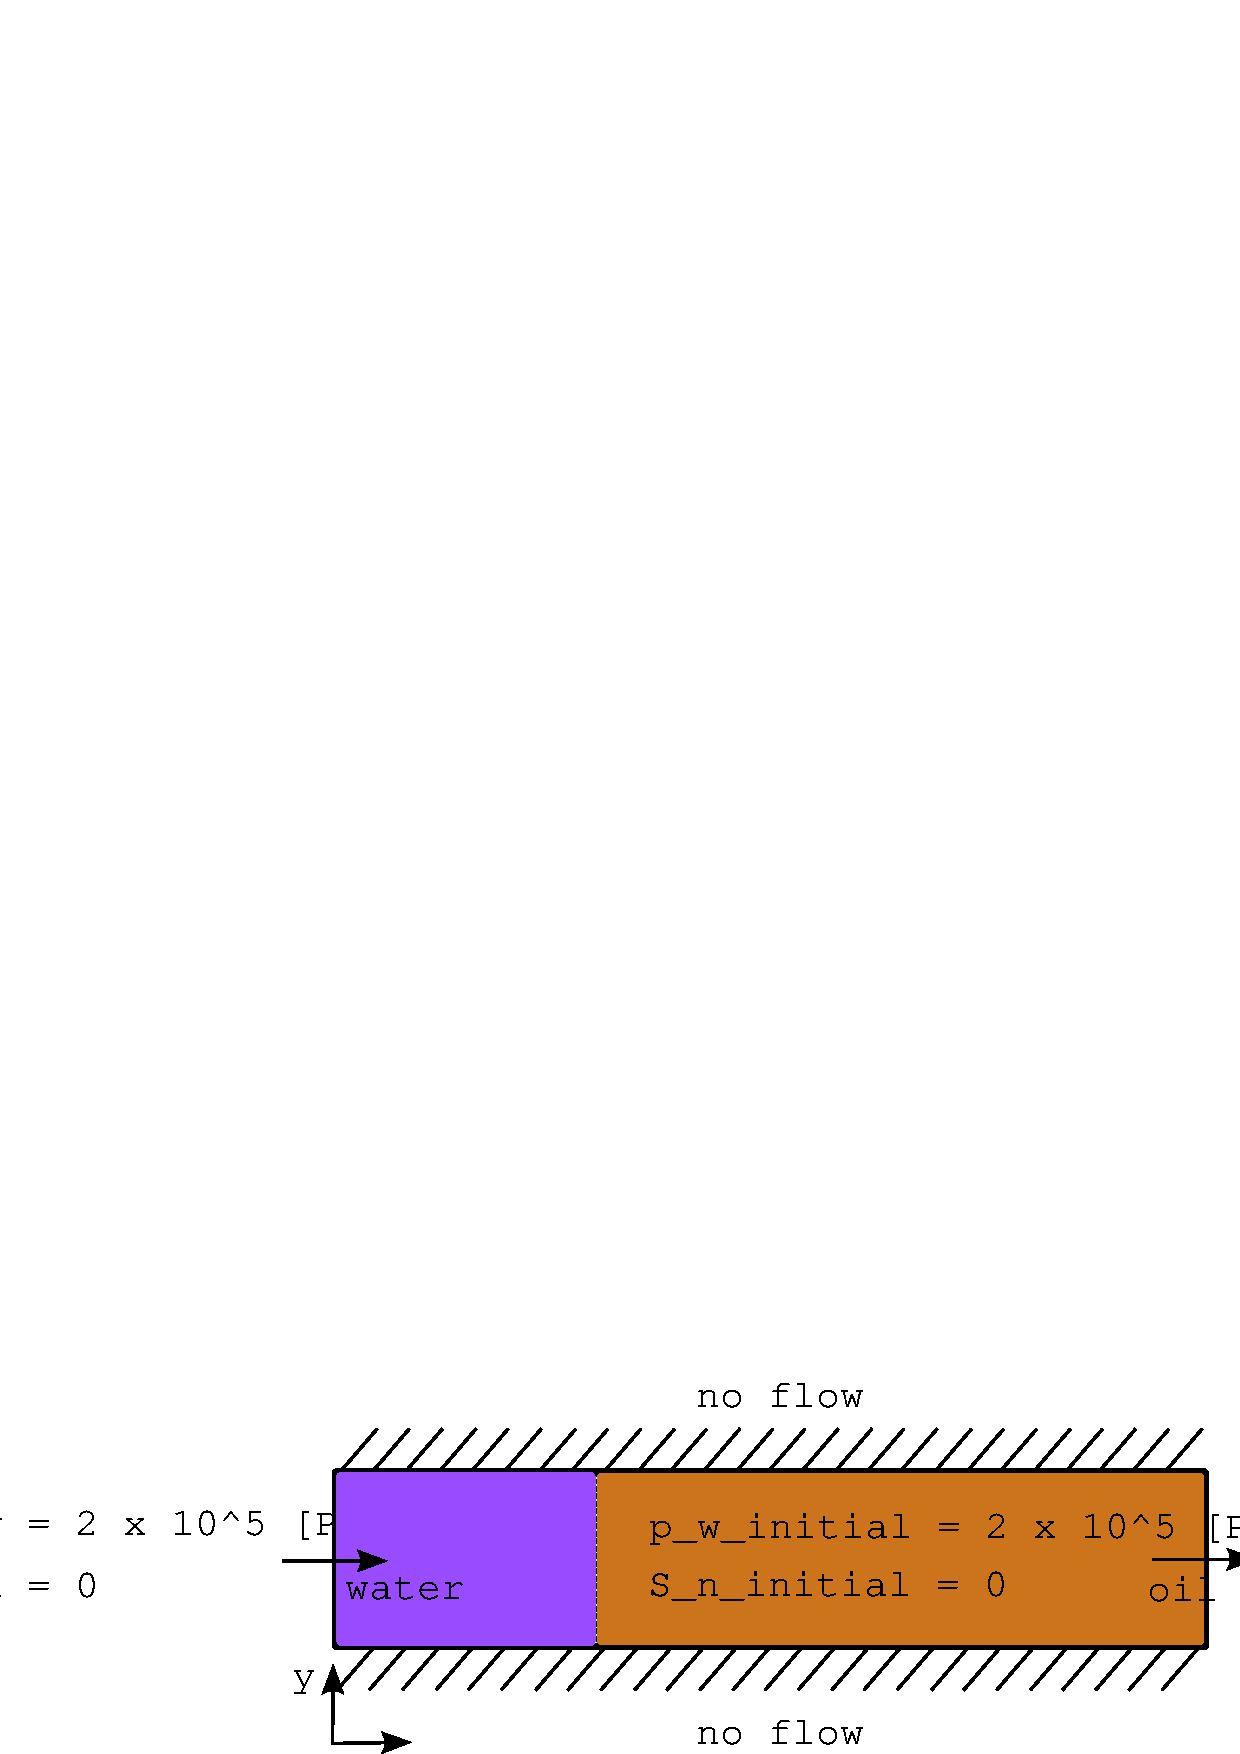
\includegraphics[width=0.9\linewidth,keepaspectratio]{EPS/tutorial-problemconfiguration}
\caption{Geometry of the tutorial problem with initial and boundary conditions.}\label{tutorial-coupled:problemfigure}
\end{figure}

The equations that are solved here are the mass balances of oil and
water:
\begin{align}
  \label{massbalancewater}
  \frac {\partial (\phi \, S_{w}\, \varrho_{w})}{\partial t}
  +
  \nabla \cdot \left( \varrho_{w} \, \frac{k_{rw}}{\mu_{w}} \, \mathbf{K}\;\nabla p \right)
  -
  q
  & =
  0 \\
  \label{massbalanceoil}
  \frac {\partial (\phi \, S_{o}\, \varrho_{o})}{\partial t}
  +
  \nabla \cdot \left( \varrho_{o} \, \frac{k_{ro}}{\mu_{o}} \, \mathbf{K}\;\nabla p \right)
  -
  q 
  & =
  0
\end{align}

\subsection{The main file}

Listing \ref{tutorial-coupled:mainfile} shows the main file
\texttt{tutorial/tutorial\_coupled.cc} for the coupled twophase
model. This file needs to be executed to solve the problem described
above.

\begin{lst}[File tutorial/tutorial\_coupled.cc]\label{tutorial-coupled:mainfile} \mbox{}
  \lstinputlisting[basicstyle=\ttfamily\scriptsize,numbers=left,
  numberstyle=\tiny, numbersep=5pt, firstline=18]{../../tutorial/tutorial_coupled.cc}
\end{lst}

From line \ref{tutorial-coupled:include-begin} to line
\ref{tutorial-coupled:include-end} the Dune and \Dumux files which
contain the needed functions and classes are included.

At line \ref{tutorial-coupled:set-type-tag} the type tag of the
problem which is going to be simulated is set. All other data types
can be retrieved by the \Dumux property system and only depend on this
single type tag. Retrieving them is done between line
\ref{tutorial-coupled:retrieve-types-begin} and
\ref{tutorial-coupled:retrieve-types-end}. For an introduction to the
property system, see section \textbf{TODO}.

The first thing which should be done at run time is to initialize the
message passing interface using DUNE's \texttt{MPIHelper} class. Line
\ref{tutorial-coupled:init-mpi} line is essential if the simulation is
intended to be run on more than one processor at the same time. Next,
the command line arguments are parsed starting at line
\ref{tutorial-coupled:parse-args-begin} until line
\ref{tutorial-coupled:parse-args-end}. In this case, we check if and
at which time a previous run of the simulation should be restarted, we
parse the initial size of a time step and the time when the simulation
ends.

After this, a grid is created on line
\ref{tutorial-coupled:create-grid} and the problem is instantiated for
its leaf grid view on line \ref{tutorial-coupled:instantiate-problem}.
Finally, on line \ref{tutorial-coupled:restart} a state written to
disk by a previous simulation run is restored on request by the user
and the simulation proceedure is started at line
\ref{tutorial-coupled:execute}.

\subsection{The problem class}

When solving a problem using \Dumux, the most important file is the
so-called \textit{problem file} as shown in listing
\ref{tutorial-coupled:problemfile} of
\texttt{tutorialproblem\_coupled.hh}.

\begin{lst}[File tutorial/tutorialproblem\_coupled.hh]\label{tutorial-coupled:problemfile} \mbox{}
\lstinputlisting[basicstyle=\ttfamily\scriptsize,numbers=left,
numberstyle=\tiny, numbersep=5pt, firstline=17]{../../tutorial/tutorialproblem_coupled.hh}
\end{lst}

First, a new type tag is created for the problem on line
\ref{tutorial-coupled:create-type-tag}.  In this case, the new type
tag inherits all properties defined for the \texttt{BoxTwoP} type tag,
which means that for this problem the two-phase box model is chosen as
discretization scheme. On line \ref{tutorial-coupled:set-problem}, a
problem class is attached to the new type tag, while the grid which
going to be used is defined on line \ref{tutorial-coupled:set-grid} --
in this case it's \texttt{SGrid}.  Since in Dune, there's no uniform
mechanism to allocate grids, the \texttt{Grid} property also contains
a static \texttt{create()} method which provides just that. Next,
fluids used as wetting phase and non-wetting phase as well as the soil
properties are specified on lines \ref{tutorial-coupled:set-wetting},
\ref{tutorial-coupled:set-nonwetting} and
\ref{tutorial-coupled:set-soil}. The final property on line line
\ref{tutorial-coupled:gravity} is optional and tells the model not to
use gravity.

Parameters which are specific to a set-up -- like boundary and initial
conditions, source terms or temperature within the domain -- but are
required to solve the differential equations of the models are
specified via a \textit{problem} class. If the two-phase box model is
used, this class must be derived from \texttt{TwoPBoxProblem} as done
on line \ref{tutorial-coupled:def-problem}.

The problem class always has at least five methods:
\begin{itemize}
\item A method \texttt{boundaryTypes()} specifying the kind of
  boundary conditions to be used for a boundary segment
\item A method \texttt{dirichlet()} specifying the actual values for
  the Dirichlet conditions on a boundary segment
\item A method \texttt{neumann()} specifying the actual values for
  the Neumann conditions on a boundary segment
\item A method for source or sink terms called \texttt{source}
\item A method called \texttt{initial()} for specifying the initial
  condition.
\end{itemize}

Methods which make statements about boundary segments of the grid (i.e. 
\texttt{boundaryTypes()}, \texttt{dirichlet()} and \texttt{neumann()}) get 
six parameters:
\begin{description}
\item[values:] A vector which stores the result of the method. What
  the values in this vector means is dependent on the method: For
  \texttt{dirichlet()} it contains the values of the primary
  variables, for \texttt{neumann()} it the mass fluxes per area unit
  over the boundary segment, and for \texttt{boundaryTypes()} it
  contains the type of boundary condition which should be used for
  each equation (either \texttt{Dune::BoundaryConditions::dirichlet} or
  \texttt{Dune::BoundaryConditions::neumann}).
\item[element:] The element of the grid where the boundary segment
  is located.
\item[fvElemGeometry:] The finite-volume geometry induced on the
  finite element by the box scheme.
\item[isIt:] The \texttt{IntersectionIterator} of the boundary
  segement as given by the grid
\item[scvIdx:] The index of the sub-control volume in
  \texttt{fvElementGeometry} adjacent to the boundary segment.
\item[boundaryFaceIdx:] The index of the boundary face in
  \texttt{fvElementGeometry} which represents the boundary segment.  
\end{description}

Similarly, the \texttt{initial()} and \texttt{dirichlet()} methods
specify properties of sub-control volumes and thus only get
\texttt{values}, \texttt{element}, \texttt{fvElemGeom} and
\texttt{scvIdx} as parameters.

In addition to these five methods, there might be some model-specific
methods. If the isothermal two-phase model is used, a
\texttt{temperature()} method which returns the temperature in Kelvin
of the fluids and the rock matrix in the domain. This temperature is
then used by the model to calculate fluid properties which possibly
depend on it, e.g. density.


\subsection{Defining fluid properties}\label{tutorial-coupled:description-fluid-class}

The \Dumux distribution includes some common fluids which can be used
out of the box. For each fluid there is a header file in
\texttt{dumux/material/fluids}, for example the fluid class for air is
located in \texttt{air.hh}. Each of these files, defines a class with
the same name as the fluid but starting with a capital letter,
e.g. \texttt{Air}. These classes are derived from \texttt{Fluid}, the
base class of all fluids in \Dumux. \texttt{Fluid} is defined in the
file \texttt{dumux/material/property\_baseclasses.hh} and features
methods returning fluid properties like density, enthalpy, viscosity,
etc. New fluids which are not yet available in the \Dumux distribution
can be defined analogous.

It is important to mention that existing fluid classes should not be
changed by the user, in order to avoid confusion. Also, new fluid
classes should only be added to the directory
\texttt{dumux/material/fluids} and if they might be useful for other
people. If you are not sure if your fluid class can be useful for
other \Dumux users, just create a new fluid in your problem directory
analogous to the ones defined in \texttt{dumux/material/fluids}.

\subsection{The definition of the soil parameters}\label{tutorial-coupled:description-soil-class}

In \Dumux, properties of the porous medium like \textit{intrinsic
  permeability}, the \textit{porosity}, the \textit{heat capacity} as
well as the \textit{heat conductivity} can be defined using a
so-called \texttt{Soil} class. Further the \textit{residual
  saturations} of the fluids, and the \textit{capillary
  pressures-saturation function} as well as the \textit{relative
  permeability-saturation functions} are defined by the soil.

The base class \texttt{Dune::Matrix2p} for the definition of the soil
parameters can be found in the file
\texttt{dumux/material/property\_baseclasses.hh}. Derived from this
base class, two standard soil types called \texttt{HomogeneousSoil}
and \texttt{HeterogeneousSoil} are included in the \Dumux
distribution, both of which are located in
\texttt{dumux/material/matrixproperties.hh}. If one wants to use a
soil that differs from this standard soil types, new soil classes can
be derived either from the base class (\texttt{Dune::Matrix2p}) or
from either \texttt{Dune::HomogeneousSoil} or
\texttt{Dune::HeterogeneousSoil}.

For this tutorial problem a new soil class named \texttt{TutorialSoil}
is derived from \texttt{Dune::HomogeneousSoil} (listing
\ref{tutorial-coupled:soilpropertiesfile}, line
\ref{tutorial-coupled:tutorialsoil}), is located in
\texttt{tutorial/tutorialsoil\_coupled.hh}.

Listing \ref{tutorial-coupled:soilpropertiesfile} shows the file
\texttt{tutorialsoil\_coupled.hh}.

\begin{lst}[File tutorial/tutorialsoil\_coupled.hh]\label{tutorial-coupled:soilpropertiesfile} \mbox{}
\lstinputlisting[basicstyle=\ttfamily\scriptsize,numbers=left,
numberstyle=\tiny, numbersep=5pt, firstline=16]{../../tutorial/tutorialsoil_coupled.hh}
\end{lst}

In line \ref{tutorial-coupled:permeability} the function returning the
intrinsic permeability can be found. As can be seen, the function has
to be called with three different arguments. The first one
(\texttt{x}) is a vector including the global coordinates of the
current entity (can be an element, vertex, etc.), the second one
(\texttt{e}) is the entity itself and the third one is a vector
including the local coordinates of the current entity. The intrinsic
permeability is a tensor and thus returned in form of a $n \times
n$-matrix where $n$ is the dimension of the problem.

The function \texttt{porosity()} defined in line
\ref{tutorial-coupled:porosity} is called with the same arguments as
the permeability function described before and returns the porosity
dependent on the position in the domain.

The residual saturation functions \texttt{Sr\_w()} (line
\ref{tutorial-coupled:srw}) and \texttt{Sr\_n()} (line
\ref{tutorial-coupled:srn}) additionally have the temperature as
function argument, which is set to a default value if an isothermal
model is used.

Finally, the functions defining the type of the capillary pressure
function and the relative permeability functions have to be
considered. In line \ref{tutorial-coupled:flags} the function
\texttt{relPermFlag()} is defined. This function returns a flag
indicating the type of function which is used depending on the
position. This could be a linear function, a \textit{Brooks-Corey}
function, a \textit{van Genuchten} function, etc. The flags that can
be chosen as return parameter are defined in the base soil class
\texttt{Matrix2p} in the file \texttt{property\_baseclasses.hh}. The
parameters used in the chosen function type can be defined in the
function \texttt{paramRelPerm} (line
\ref{tutorial-coupled:parameters}). As can be seen in listing
\ref{tutorial-coupled:soilpropertiesfile}, e.g. linear capillary
pressure and relative permeability functions require a vector of two
arguments, one defining the minimum and one defining the maximum
capillary pressure. The parameters can again be defined depending on
the position in the domain an on temperature.

\subsection{Exercises}
\label{tutorial-coupled:exercises}
The following exercises will give you the opportunity to learn how you
can change soil parameters, boundary conditions and fluid properties
in \Dumux. For each exercise you can find the output file of the last
timestep in the directory \texttt{tutorial/results/coupled}.

\subsubsection{Exercise 1}
\renewcommand{\labelenumi}{\alph{enumi})} For Exercise 1 you only have
to make some small changes in the tutorial files.  To get an
impression what the results should look like you can first run the
original version of the fully-coupled tutorial model by typing
\texttt{./tutorial\_coupled}. For the visualisation with paraview
please refer to \ref{quick-start-guide}.
\begin{enumerate}
\item \textbf{Changing the Model Domain and the Boundary Conditions} \\

  Change the size of the model domain so that you get a rectangle with
  edge lengths of $\text{x} = 400 m$ and $\text{y} = 500 m$ and with
  discretization lengths of $\Delta \text{x} = 20$ m and $\Delta
  \text{y} = 20$ m.
  
  Change the boundary conditions in the file
  \texttt{tutorialproblem\_coupled.hh} so that water enters from the
  bottom and oil is extracted from the top boundary. The right and the
  left boundary should be closed for water and oil fluxes. 

  Compile the main file by typing \texttt{make tutorial\_coupled} and
  run the model.


\item \textbf{Changing Fluids} \\
  Now you can change the fluids. Use \texttt{DNAPL} instead of
  \texttt{Oil} and \texttt{Brine} instead of \texttt{Water}. To do
  that you have to change the problem file
  \texttt{tutorialproblem\_coupled.hh}. If you want to take a closer
  look how the fluid classes are defined and which fluids are already
  available please open the file \texttt{dumux/material/fluids/air.hh}
  for an example.


\item \textbf{Changing Constitutive Relations} \\
  Use a Brooks-Corey law with $\lambda = 2$ and entry pressure $p_e =
  0.0$ instead of using a linear law for the
  relative-permeability/saturation relationship. To do that you have
  to change the file \texttt{tutorialsoil\_coupled.hh}. You can find
  the flag that you have to set for the Brooks-Corey law in the file
  \texttt{dumux/material/property\_baseclasses.hh}.  The available
  relative permeability and capillary pressure functions are defined
  in the file \texttt{/dumux/material/relperm\_pc\_law}.
 
\item \textbf{Heterogeneities}  \\
  Set up a model domain with the soil properties given in Figure
  \ref{tutorial-coupled:exercise1_d}. Adjust the boundary conditions
  so that water is still flowing from the bottom to the top of the
  domain. You can use the fluids of exercise 1b) and the constitutive
  relationship of exercise 1c).

\begin{figure}[h]
\psfrag{K1 =}{K $= 10^{-8}\text{ m}^2$}
\psfrag{phi1 =}{$\phi = 0.15$}
\psfrag{K2 =}{\textcolor{white}{K $= 10^{-9}\text{ m}^2$}}
\psfrag{phi2 =}{\textcolor{white}{$\phi = 0.3$}}
\psfrag{600 m}{600 m}
\psfrag{300 m}{300 m}
\centering
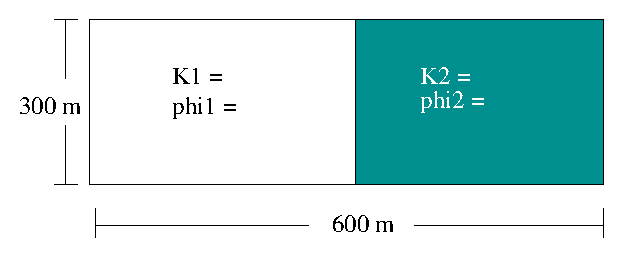
\includegraphics[width=0.5\linewidth,keepaspectratio]{EPS/exercise1_c.eps}
\caption{Exercise 1d: Set-up of a model domain a heterogeneity. $\Delta \text{x} = 20$ m $\Delta \text{y} = 20$ m.}\label{tutorial-coupled:exercise1_d}
\end{figure}

\end{enumerate}

\subsubsection{Exercise 2}
For this exercise you should create a new proplem file analogous to
the file \texttt{tutorialproblem\_coupled.hh} and a new soil property
file just like \texttt{tutorialsoil\_coupled.hh}. These files need to
be included in the file \texttt{tutorial\_coupled.cc}. 

The new soil file should contain the definition of a new soil class
e.g. \texttt{SoilEx2}. Make sure that you also adjust the guardian
macros in the header files (e.g. change \texttt{TUTORIAL\_SOIL} to
\texttt{TUTORIAL\_SOILEX2}).  The new problem file should define and
use a new type tag for the problem as well as a new problem class
e.g. \texttt{ProblemEx2}. Make sure you assign your newly defined soil
class to the \texttt{Soil} property for the new type tag. Just like
for your new soil, you also need to adjust the guardian macros in the
problem file.

After this, change the \texttt{create()} method of the \texttt{Grid}
property and your soil class, so that it matches the domain described
by figure \ref{tutorial-coupled:ex2_Domain}. Adapt the problem class
so the boundary conditions are consistent with figure
\ref{tutorial-coupled:ex2_BC}. Initially the domain is fully saturated
with water and the pressure is $p_w = 5 \times 10^5 \text{Pa}$ . Oil
infiltrates from the left side. Create a grid with $20$ cells in
$x$-direction and $10$ cells in $y$-direction. The simulation time
should be set to $4\times 10^7 \text{s}$ with an inital time step of
$100 \text{s}$.

Now include your new problem file in the main file and replace the
\texttt{TutorialProblemCoupled} type tag by the one you've created and
compile the program.


\begin{figure}[h]
\psfrag{K1}{K $= 10^{-7}\text{ m}^2$}
\psfrag{phi1}{$\phi = 0.2$}
\psfrag{Lin}{Linear Law}
\psfrag{K2}{K $= 10^{-9}\text{ m}^2$}
\psfrag{phi2}{$\phi = 0.15$}
\psfrag{BC1}{Brooks Corey Law} 
\psfrag{BC2}{$\lambda = 1.8$, $p_b = 0.0$}
\psfrag{H1y}{50 m}
\psfrag{H2y}{15 m}
\psfrag{H3y}{20 m}
\psfrag{L1x}{100 m}
\psfrag{L2x}{50 m}
\psfrag{L3x}{25 m}
\centering
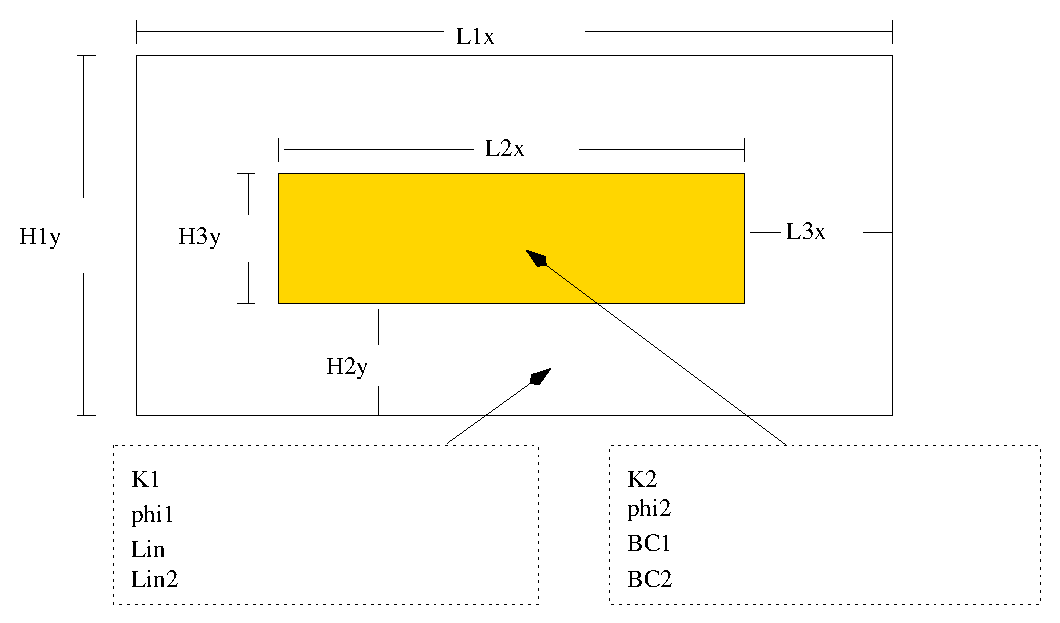
\includegraphics[width=0.8\linewidth,keepaspectratio]{EPS/Ex2_Domain.eps}
\caption{Set-up of the model domain and the soil parameters}\label{tutorial-coupled:ex2_Domain}
\end{figure}

\begin{figure}[h]
\psfrag{pw}{$p_w = 5 \times 10^5$ \text{Pa}}
\psfrag{S}{$S_n = 1.0$}
\psfrag{qw}{$q_w = 2 \times 10^{-4}$ [kg/$\text{m}^2$s]}
\psfrag{qo}{$q_n = 0.0$ [kg/$\text{m}^2$s]}
\psfrag{no flow}{no flow}
\centering
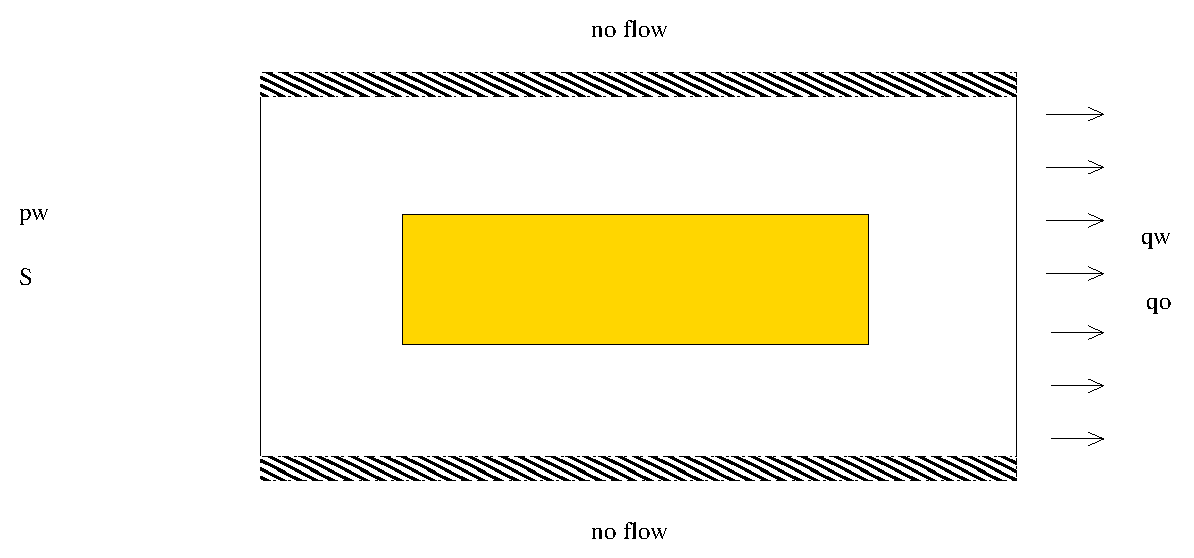
\includegraphics[width=0.8\linewidth,keepaspectratio]{EPS/Ex2_Boundary.eps}
\caption{Boundary Conditions}\label{tutorial-coupled:ex2_BC}
\end{figure}

\subsubsection{Exercise 3}

Create a new file for benzene called \texttt{benzene.hh} and implement
a new fluid class. This new fluid class should be derived from the
base class \texttt{Fluid} located in
\texttt{/dumux/material/property\_baseclasses.hh}.  (You may get a
hint by looking at existing fluid classes in the directory
\texttt{/dumux/material/fluids}.)

Use benzene as a new fluid and run the model of Exercise 2 with water
and benzene. Benzene has the following properties:
\begin{description}
  \item[density:] $889.51 \, \text{kg} / \text{m}^3$
  \item[viscosity:] $0.00112 \, \text{Pa} \; \text{s}$
\end{description}


\clearpage
\section[Decoupled model]{Solving a problem using a Decoupled Model}\label{tutorial-decoupled}

The process of solving a problem using \Dumux can be roughly divided into four parts: 
\begin{enumerate}
 \item The geometry of the problem and correspondingly a grid have to be defined.
 \item Material properties and constitutive relationships have to be defined.
 \item Boundary conditions as well as initial conditions have to be defined.
 \item A suitable model has to be chosen.
\end{enumerate}

The problem which is solved in this tutorial is illustrated in figure \ref{tutorial-decoupled:problemfigure}. A rectangular domain with now flow boundaries on the top and at the bottom, which is initially saturated with oil, is considered. Water infiltrates from the left side into the domain. Gravity effects as well as capillarity effects are neglected.

\begin{figure}[h]
\psfrag{x}{x}
\psfrag{y}{y}
\psfrag{no flow}{no flow}
\psfrag{water}{water}
\psfrag{oil}{oil}
\psfrag{p_w = 2 x 10^5 [Pa]}{$p_w = 2 \times 10^5$ [Pa]}
\psfrag{p_w_initial = 2 x 10^5 [Pa]}{$p_{w_{initial}} = 2 \times 10^5$ [Pa]}
\psfrag{S_n = 0}{$S_n = 0$}
\psfrag{S_n_initial = 0}{$S_{n_{initial}} = 0$}
\psfrag{q_w = 0 [kg/m^2s]}{$q_w = 0$ $\left[\frac{\textnormal{kg}}{\textnormal{m}^2 \textnormal{s}}\right]$}
\psfrag{q_n = -3 x 10^-4 [kg/m^2s]}{$q_w = -3 \times 10^-4$ $\left[\frac{\textnormal{kg}}{\textnormal{m}^2 \textnormal{s}}\right]$}
\centering
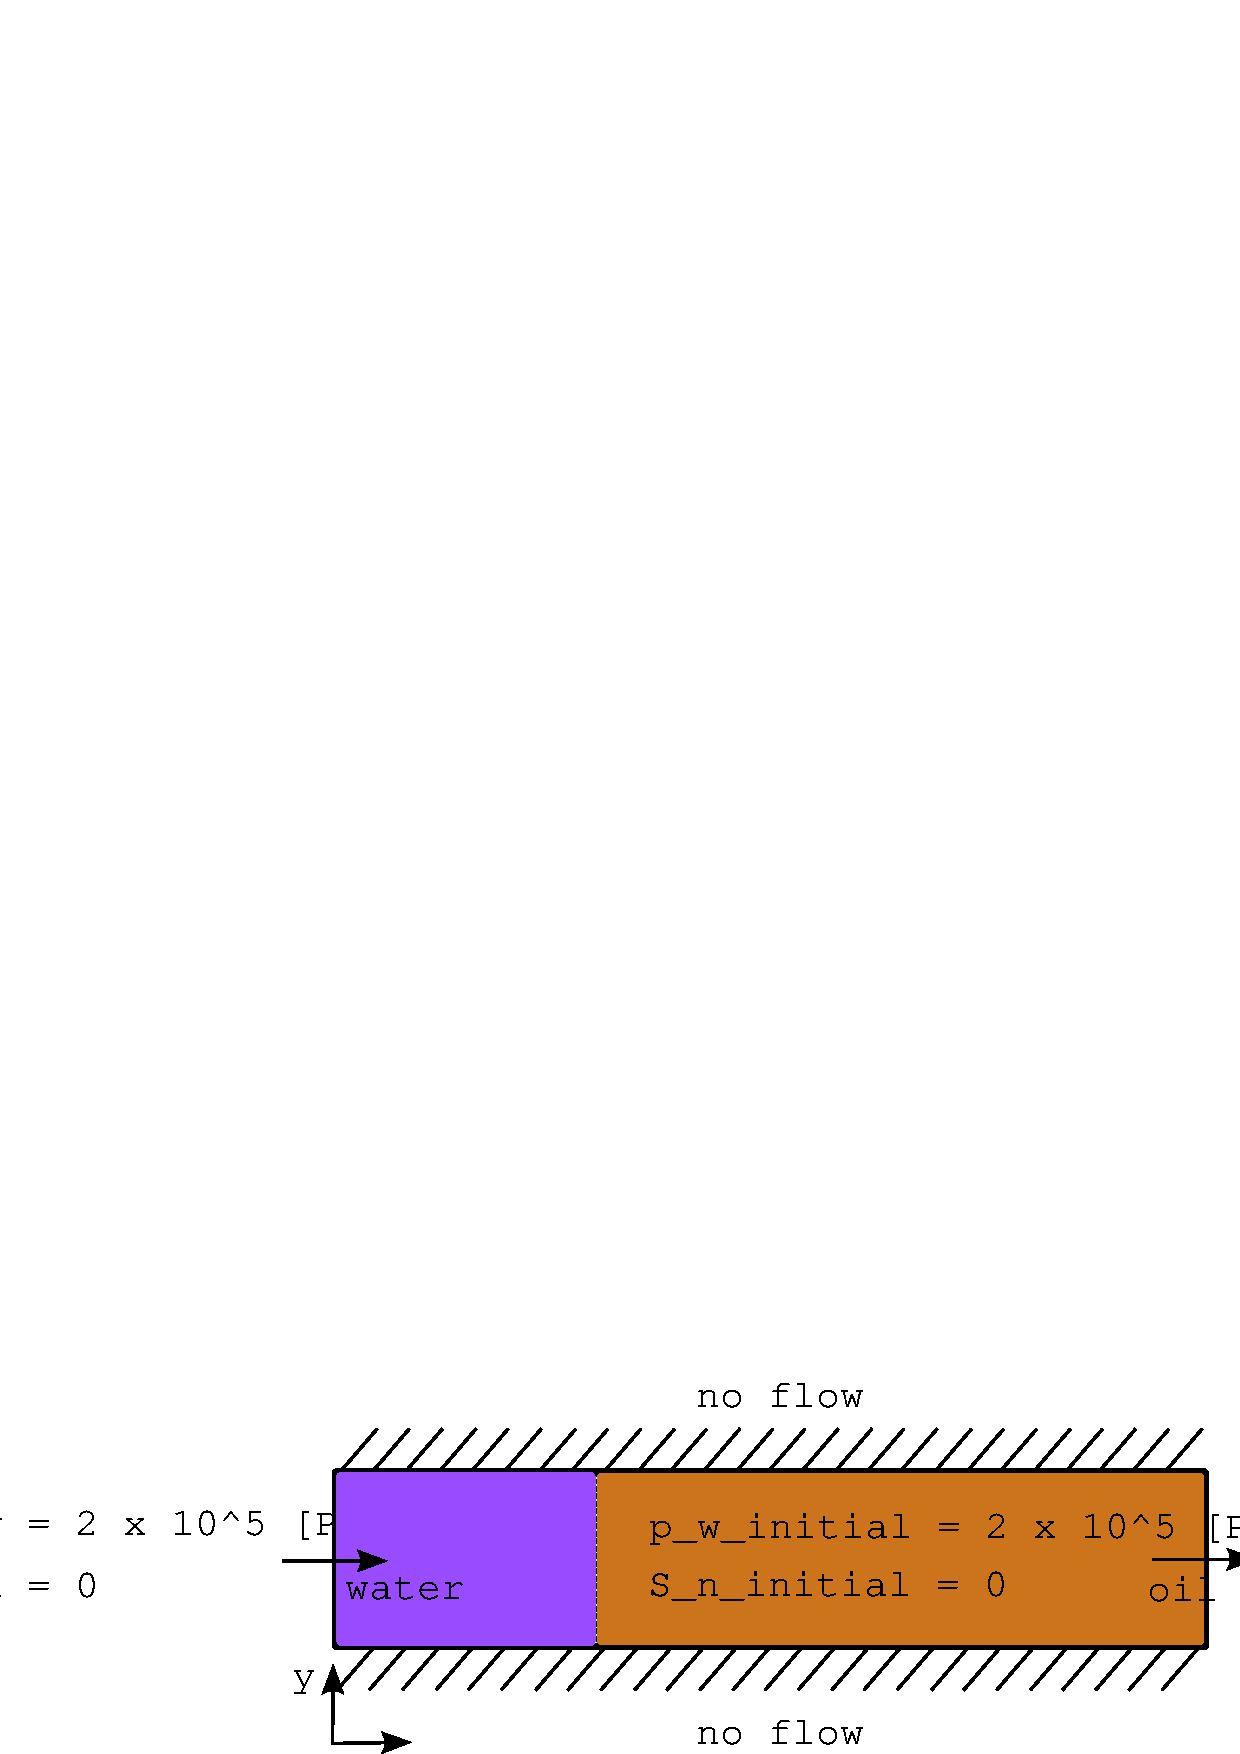
\includegraphics[width=0.9\linewidth,keepaspectratio]{EPS/tutorial-problemconfiguration}
\caption{Geometry of the tutorial problem with initial and boundary conditions.}\label{tutorial-decoupled:problemfigure}
\end{figure}

Listing \ref{tutorial-deoucpled:mainfile} shows how the main file, which has to be executed, has to be set up, if the problem described above is to be solved using a decoupled model. This main file can be found in the directory \texttt{/dune-mux/test/tutorial}.

\begin{lst}[File dune-mux/test/tutorial/tutorial\_decoupled.cc]\label{tutorial-deoucpled:mainfile} \mbox{}
\lstinputlisting[basicstyle=\ttfamily\scriptsize,numbers=left, 
numberstyle=\tiny, numbersep=5pt]{../../test/tutorial/tutorial_decoupled.cc}
\end{lst}

First, in line \ref{tutorial-decoupled:include-begin} to \ref{tutorial-decoupled:include-end} the Dune and the \Dumux files respectively which contain the functions and classes that are needed in the main loop are included into the main file.

In line \ref{tutorial-decoupled:grid-begin} to \ref{tutorial-decoupled:grid-end} the geometry is defined and the grid is generated. The three variables of Type \texttt{Dune::FieldVector} define the lower left corner of the domain (\texttt{L}), the upper right corner of the domain (\texttt{H}) and the number of cells in $x$ and $y$ direction (\texttt{N}), where the dimensions are previously defined in line \ref{tutorial-decoupled:dim}. The grid of type \texttt{Dune::SGrid} is then generated in line \ref{tutorial-decoupled:grid-end}. For more information about the dune grid interface, the different grid types that are supported and the generation of different grids it is referred to the \textit{Dune Grid Interface HOWTO} (REFERENCE!!!).

The second point mentioned at the beginning of this section was the definition of material properties and constitutive relationships. The fluid properties of the two fluid phases considered here are defined in lines \ref{tutorial-decoupled:water} and \ref{tutorial-decoupled:oil}. The fluid classes including different kinds of fluids (here: \texttt{Dune::Water} and \texttt{Dune::Oil}) can be found in the file \texttt{phaseproperties2p.hh} in the directory \texttt{/dune-mux/dumux}-\texttt{/material/phaseproperties}. The properties of the solid matrix are defined in a special soil class. The \texttt{soil} object is generated in line \ref{tutorial-decoupled:soil}. As can be seen, the class type is \texttt{Dune::TutorialSoil}, which is defined in the file \texttt{tutorial\_soilproperties.hh} in the folder \texttt{/test/tutorial}. A description of this file and the definition of a soil class including the soil parameters can be found in section \ref{tutorial-decoupled:description-soil-class}. Finally, in line \ref{tutorial-decoupled:twophaserelations} the information included in the fluid and soil objects is used to generate an object of type \texttt{Dune::TwoPhaseRelations}, which includes the constitutive relationships (capillary pressure-saturation relation, relative permeability-saturation relation, etc.). The file \texttt{twophaserelations.hh} can be found in the directory \texttt{/dune-mux/dumux/material}.

The definition of boundary and initial conditions as well as source of sink terms is done by definition of a so-called \textit{problem} class. In case of this tutorial the problem class is defined in the file \texttt{tutorialproblem\_decoupled.hh} in the \texttt{/test/tutorial} folder. In the main file the problem object of type \texttt{Dune::TutorialProblemDecoupled} is then generated in line \ref{tutorial-decoupled:problem}. A further explanation of the definition of boundary and initial conditions, source and sink terms and the structure of the problem class can be found in section \ref{tutorial-decoupled:description-bc-ic}. Besides the definition of the boundary and initial conditions the problem class is also a kind of interface containing all the objects generated before (geometry, fluids, soil, constitutive relationships, etc.). Thus, as can be seen in line \ref{tutorial-decoupled:problem} all this objects are given as arguments when calling the constructor of the problem class.

Following the steps listed at the beginning of this section, finally, a model has to be chosen. In case of this tutorial a decoupled isothermal two phase model is the choice. As explained before a decoupled model consists of a pressure equation which is decoupled or only weakly coupled to a saturation equation, concentration equations, energy balance equations, etc. In case of isothermal two phase flow one pressure equation and one saturation equation have to be solved. 

The discretisation of the pressure equation is included in the object which is generated in line \ref{tutorial-decoupled:diffusion} of the main file. It is called \texttt{diffusion} and it is of type \texttt{Dune::FVDiffusionVelocity}. The definition of this class can be found in \texttt{/dune-mux/dumux/diffusion/fv} in the file \texttt{fvdiffusionvelocity.hh}. The \texttt{FV} in the class name indicates that a \textit{finite volume} discretisation is used. For the pressure equation also other discretisation methods like \textit{finite elements} or \textit{mimetic finite differences} are available.

Similarly, an object containing the discretisation of the saturation equation is generated in line \ref{tutorial-decoupled:transport} of the main file. As can be seen, this object is called \texttt{transport}. The class  \texttt{Dune::FVTransport} can be found in the directory \texttt{/dune-mux/dumux/transport/fv}. Again, the \texttt{FV} in the class name indicates a \textit{finite volume} discretisation.

For the decoupled model the so-called \textit{IMPES} (\textit{IM}plicit \textit{P}ressure \textit{E}xplicit \textit{S}aturation) algorithm is used. This means that the pressure equation is first solved using an implicit method. The resulting velocities are then used to solve the saturation equation explicitly. It is clear that depending on the non-linearity this is an iterative process within every timestep. The object \texttt{impes} of type \texttt{Dune::IMPES} which is generated in line \ref{tutorial-decoupled:impes} of the main file combines the objects \texttt{diffusion} and \texttt{transport} and proceeds the iterations of the IMPES algorithm within a timestep. The definition of the class \texttt{Dune::IMPES} can be found in the file \texttt{impes.hh} in the directory \texttt{/dune-mux/dumux/fractionalflow/impes}.

Finally, an object called \texttt{timeloop} of type \texttt{Dune::TimeLoop} is generated in line \ref{tutorial-decoupled:timeloop} of the tutorial main file. The class \texttt{Dune::TimeLoop} is defined in the file \texttt{timeloop.hh} in the folder \texttt{/dune-mux/dumux/timedisc}. The object \texttt{timeloop} includes the type of timestep that is used (implicit, explicit, etc.) and contains the function \texttt{execute} which is called in line \ref{tutorial-decoupled:execute} of the main file. This function finally starts the computation and runs the (time)loop over all timesteps.

\subsection{The definition of the fluid properties}\label{tutorial-decoupled:description-fluid-class}

In \Dumux different fluids are already implemented. The definitions can be found in the file \texttt{phaseproperties2p.hh} in the directory \texttt{/dune-mux/dumux/material/phaseproperties}. As can be observed in this file, for each fluid a class named like the fluid is defined. These classes are derived from the fluid base class \texttt{Fluid} which is defined in the file \texttt{property\_baseclasses.hh} in the directory \texttt{/dune-mux/dumux/material} and include several functions returning different fluid properties.

If a new fluid type is to be used or an existing type is to be used with different fluid parameters new fluid types can be defined derived from the base class \texttt{Fluid} comparable to the fluids already defined in the file \texttt{phaseproperties2p.hh}.

It is important to mention, that existing fluid classes should not be changed. New fluid classes should only be added to the file \texttt{phaseproperties2p.hh} if they are also to be added to the repository! If you are not sure if your fluid class can be useful for the other \Dumux users just create a new file in your problem directory similar to the file \texttt{phaseproperties2p.hh} and define your fluid classes there. 

\subsection{The definition of the soil parameters}\label{tutorial-decoupled:description-soil-class}

Soil properties which can be defined in \Dumux are the \textit{intrinsic permeability}, the \textit{porosity} and the \textit{heat capacity} as well as the \textit{heat conductivity} of the solid matrix. Further the \textit{residual saturations} of the fluids, and the \textit{capillary pressures-saturation function} as well as the \textit{relative permeability-saturation functions} are depending on the soil.

The base class \texttt{Dune::Matrix2p} for the definition of the soil parameters can be found in the file \texttt{property\_baseclasses.hh} in the directory \texttt{/dune-mux/dumux/material}. Derived from this base class, there exist two standard soil type classes named \texttt{HomogeneousSoil} and \texttt{HeterogeneousSoil}. Both can be found in the file \texttt{matrixproperties.hh} in the \texttt{/material} folder. If one wants to use a soil that differs from this standard soil types, new soil classes can be derived either from the base class (\texttt{Dune::Matrix2p}) or from the two standard soil classes (\texttt{Dune::HomogeneousSoil} and \texttt{Dune::HeterogeneousSoil}).

For this tutorial problem a new soil class named \texttt{TutorialSoil} is derived from \texttt{Dune::HomogeneousSoil} (listing \ref{tutorial-deoucpled:soilpropertiesfile}, line \ref{tutorial-decoupled:tutorialsoil}), which can be found in the file \texttt{tutorial\_soilproperties.hh} in the directory \texttt{/test/tutorial}.

Listing \ref{tutorial-deoucpled:soilpropertiesfile} shows the file \texttt{tutorial\_soilproperties.hh}.

\begin{lst}[File dune-mux/test/tutorial/tutorial\_soilproperties.hh]\label{tutorial-deoucpled:soilpropertiesfile} \mbox{}
\lstinputlisting[basicstyle=\ttfamily\scriptsize,numbers=left, 
numberstyle=\tiny, numbersep=5pt]{../../test/tutorial/tutorial_soilproperties.hh}
\end{lst}

In line \ref{tutorial-decoupled:permeability} the function returning the intrinsic permeability can be found. As can be seen, the function has to be called with three different arguments. The first one (\texttt{x}) is a vector including the global coordinates of the current entity (can be an element, vertex, etc.), the second one (\texttt{e}) is the entity itself and the third one is a vector including the local coordinates of the current entity. The intrinsic permeability is a tensor and thus returned in form of a $n \times n$-matrix where $n$ is the dimension of the problem.

The function \texttt{porosity()} defined in line \ref{tutorial-decoupled:porosity} is called with the same arguments as the permeability function described before and returns the porosity dependent on the position in the domain.

The residual saturation functions \texttt{Sr\_w()} (line \ref{tutorial-decoupled:srw}) and \texttt{Sr\_n()} (line \ref{tutorial-decoupled:srn}) additionally have the temperature as function argument, which is set to a default value if a isothermal model is used.

Finally, the functions defining the type of the capillary pressure function and the relative permeability functions have to be considered. In line \ref{tutorial-decoupled:flags} the function \texttt{relPermFlag()} is defined. This function returns a flag indicating the type of function which is used depending on the position. This could be a linear function, a \textit{Brooks-Corey} function, a \textit{van Genuchten} function, etc. The flags that can be chosen as return parameter are defined in the base soil class \texttt{Matrix2p} in the file \texttt{property\_baseclasses.hh}. The parameters used in the chosen function type can be defined in the function \texttt{paramRelPerm} (line \ref{tutorial-decoupled:parameters}). As can be seen in listing \ref{tutorial-deoucpled:soilpropertiesfile}, e.g. linear capillary pressure and relative permeability functions require a vector of two arguments, one defining the minimum and one defining the maximum capillary pressure. The parameters can again be defined depending on the position in the domain an on temperature.

\subsection{The definition of boundary and initial conditions and source or sink terms}\label{tutorial-decoupled:description-bc-ic}

Boundary and initial conditions are defined in a so-called problem class. The problem class of this tutorial has the name \texttt{TutorialProblemDecoupled} and is defined in the file \texttt{tutorialproblem\_decoupled.hh} which can be found in the directory \texttt{/test/tutorial}. Listing \ref{tutorial-deoucpled:problemfile} shows the class \texttt{TutorialProblemDecoupled}. As can be seen it is derived from the problem base class \texttt{FractionalFlowProblem} (line \ref{tutorial-decoupled:tutorialproblem}) which is defined in the file \texttt{fractionalflowproblem.hh} in the directory \texttt{/dune-mux/dumux/fractionalflow}. 

\begin{lst}[File dune-mux/test/tutorial/tutorialproblem\_decoupled.hh]\label{tutorial-deoucpled:problemfile} \mbox{}
\lstinputlisting[basicstyle=\ttfamily\scriptsize,numbers=left, 
numberstyle=\tiny, numbersep=5pt]{../../test/tutorial/tutorialproblem_decoupled.hh}
\end{lst}

Listing \ref{tutorial-decoupled:tutorialproblem}) includes five types of functions. The type of each function can be identified by the first letter and the first part respectively of its name. Function names of functions returning
\begin{itemize}
 \item a source or sink term start with a \textbf{q},
 \item a boundary condition type start with \textbf{bctype},
 \item a \textit{Dirichlet} boundary condition start with a \textbf{g},
 \item a \textit{Neumann} boundary condition start with a \textbf{J} and
 \item a initial condition start with \textbf{init}. 
\end{itemize}
The second part of the function name indicates if the return value is used for the pressure equation (\textbf{Press}) or for the saturation equation (\textbf{Sat}).

All different function types have to be called with three different arguments. The first one (\texttt{x}) is a vector including the global coordinates of the current entity (can be an element, vertex, etc.), the second one (\texttt{e}) is the entity itself and the third one is a vector including the local coordinates of the current entity. Thus, the return of the functions, which can be a boundary value, an initial value, a source/sink, etc., can be defined depending on the position in the domain.

The first function defined in the problem class \texttt{TutorialProblemDecoupled} is the function \texttt{qPress} (line \ref{tutorial-decoupled:qpress}). It returns a source or a sink term for the pressure equation. 

In lines \ref{tutorial-decoupled:bctypepress} and \ref{tutorial-decoupled:bctypesat} the functions returning the boundary condition type are defined. Flags of type \texttt{Dune::BoundaryConditions::Flags} have to be used as return value of these functions. The flags that can be chosen are defined in the file \texttt{boundaryconditions.hh} in the directory \texttt{/dune-disc/disc/operators}.

In lines \ref{tutorial-decoupled:gpress} and \ref{tutorial-decoupled:gsat} the functions returning the \textit{Dirichlet} boundary conditions and in line \ref{tutorial-decoupled:jpress} a function returning the \textit{Neumann} boundary conditions are defined.

Finally, the function \texttt{initSat} is defined in line \ref{tutorial-decoupled:initsat}. This function returns the initial saturation distribution.

\subsection{Exercise}
TODO: give some exercises
\section[New model]{How to implement a new model}

TODO: describe how to impelment a new model

\bibliographystyle{plain}
%\bibliography{dumux-handbook}

\printindex

\end{document}
